\chapter{研究方法}
  本课题主要目的是为了着重在实时性方面进行主要的研究。所以总的研究采用了横向比较的思路,即在各个不同的解决方案如RDBMS和NOSQL之间进行控制变量的比较。整个比较的过程分为基础性的调研,并在实验的基础上得出结论。而后根据实验的结果进行实时性上的优化。采取各种各样的方法力图将每一个查询处理所用到的延迟时间降到最低,以期满足性能上的要求。


  基础性调研具体来说就是将相同的查询应用到同一数据上进行对比。这里的查询包括常见的简单查询和复杂查询,如连接查询;这里的数据分为小数量级和大数量级;这里的比较内容主要是查询所消耗的时间,即实时性指标;这里的比较是在mysql、hive、hbase和mongoDB之间。

  
  改进的过程具体来说就是充分发挥各个开源产品的优点,能够分布式的进行分布式查询,能够将表结构进行优良设计的进行优良设计,能够修改相关参数的争取把参数调到最优,能够改进实现算法的改进实现算法。以完成查询处理的最佳实践。


\section{Hive和HBase的整合}
  由于非关系型数据库hbase不提供条件查询的接口,但是作为一个面向列簇的NOSQL数据库它又具有自己独特的优点。为了能够较为方便的实现HBase的条件查询,考虑到hive的查询引擎使用的方便性,我们这里利用到了apache Hbase官方网站\footnote{http://wiki.apache.org/hadoop/Hive/HBaseIntegration
}上提供的整合工具hive-hbase-handler.jar实现二者的整合。

\subsection{原理}
图2-1是这种方法的实现原理。


\begin{figure}[!ht]
\centering
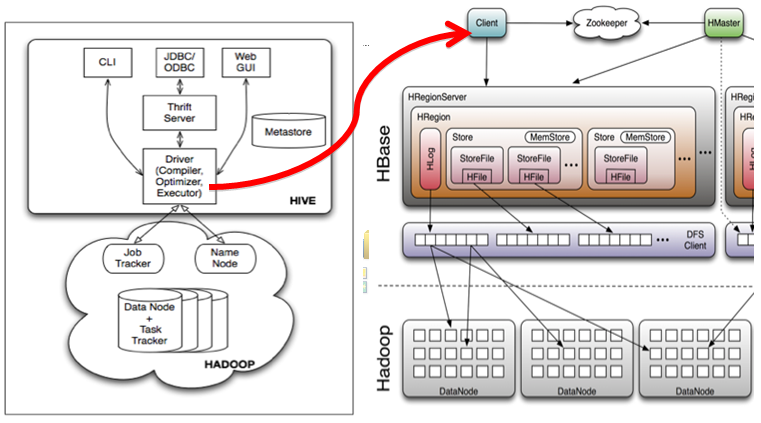
\includegraphics[scale=0.8]{photo/hive-hbase.PNG} 
\caption{Hive和HBase整合的原理}
\end{figure} 


  如图所示,左边的部分是hive的架构图,之前的hive是直接建立在Hadoop集群之上的,也就是说hive作为一个查询引擎驱动直接操作HDFS中存放的数据。而现在可以将Hive作为Hbase的client,这样一来就能够通过hive来实现数据的条件查询,复杂查询等等,另一方面数据还是存在HBase中的。总体的效果就是hive中插入的数据无论在hive还是在hbase中都能看到而且效果一样。同理,在hbase中修改数据后在Hive中查询得到的结果也会随之改变。

\subsection{整合的过程}
\begin{enumerate}
\item 将hbase-0.90.5.jar和zookeeper-3.3.2.jar拷贝到hive/lib下。
注意:如何hive/lib下已经存在这两个文件的其他版本(例如zookeeper-3.3.1.jar),建议删除后使用hbase下的相关版本。


拷贝hbase-site.xml到hive/conf目录下(我在没拷贝时出现过hbase master not running exception,拷贝后就好了)。

拷贝hbase/conf下的hbase-site.xml文件到所有hadoop节点(包括master)的hadoop/conf下。

这一部分就是通过拷贝配置文件使得hive和hbase互相了解对方的版本和具体的配置细节,以便于handler调用。

\item 在\$HIVE\_HOME/conf 目录中修改文件hive-site.xml:

\begin{figure}[!ht]
\centering
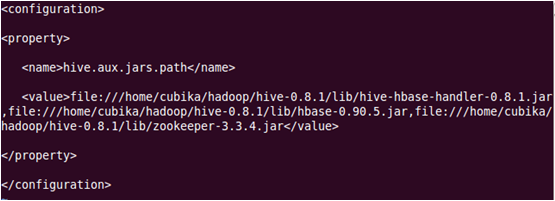
\includegraphics[]{photo/hive-site.PNG} 
\caption{hive-site.xml的设置}
\end{figure} 

如图所示,就是在启动时提供了各个jar包的路径用来加载。

\item 单节点启动方法:
bin/hive –hiveconf hbase.master=master:60000
集群启动方法:
bin/hive –hiveconf hbase.zookeeper.quorum=slave


\item  创建hbase识别的数据库:

\begin{lstlisting}[language=SQL]
CREATE TABLE hbase_table_1(key int, value string)  
STORED BY 'org.apache.hadoop.hive.hbase.HBaseStorageHandler'  
WITH SERDEPROPERTIES ("hbase.columns.mapping" = ":key,cf1:val")  
TBLPROPERTIES ("hbase.table.name" = "xyz");
\end{lstlisting}


这里主要的两点是:1.存储时用到了HBaseStorageHandler,这个工具的作用就是可以用它来创建和操作新的HBase表格。2.指定时加入映射的关系,即hbase.columns.mapping,将hive表中的某一列映射为hbase的某一列族的某一列,在指定时要明确用:key来使某一列称为Hbase的rowkey,另外映射前后表的列数必须相同。

\item 导入数据

\begin{lstlisting}[language=SQL]
hive> CREATE TABLE pokes (foo INT, bar STRING); 
hive> LOAD DATA LOCAL INPATH './examples/files/kv1.txt' OVERWRITE INTO TABLE pokes;
hive> INSERT OVERWRITE TABLE hbase_table_1 SELECT * FROM pokes WHERE foo=86;
\end{lstlisting}

这样就在整合的表hbase\_table\_1中插入了一条记录。

\item 分别在hive中和hbase中查看数据

在hive中查看:
\begin{lstlisting}[language=SQL]
hive> select * from  hbase_table_1;
\end{lstlisting}

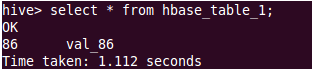
\includegraphics[]{photo/integration-hive.png}

在hbase中查看:
\begin{lstlisting}[language=SQL]
hbase(main):001:0> describe 'xyz'   
hbase(main):002:0> scan 'xyz'
\end{lstlisting}

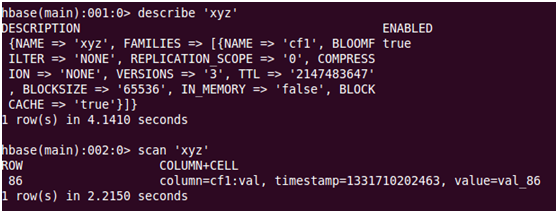
\includegraphics[]{photo/integration-hbase.png}

  从上两幅图中可以看出,经过整合之后的确能在hive里面查询hbase表格中存在的数据。说明二者已经紧密结合。
\end{enumerate}

\section{数据导入}
在基础性调研之前需要进行各个表格的创建以及数据的导入。数据的导入方法随着数据库的不同而不同,导入的时间消耗其实也可以作为一项实时性的性能指标。

\subsection{将数据导入到hive}
  这里导入的文件格式是csv -- 逗号分隔型取值格式(英文全称为Comma Separated Values,简称CSV)。它是一种纯文本格式,用来存储数据。在CSV中,数据的字段由逗号分开,程序通过读取文件重新创建正确的字段。下面介绍导入的具体步骤。

\begin{enumerate}

\item 从https://github.com/ogrodnek/csv-serde 下载hive导入csv的serde包,在hive里将这个包的路径添加进来: add jar /home/cloud/csv-serde-1.1.2.jar。有了这个jar包才能进行csv格式文本的导入工作。

\item 创建表bicc
这是一个电信的表格,每一项是一宗通话的各个具体的信息。建表语句为:

\begin{lstlisting}[language=SQL]
CREATE TABLE bicc
(
  START_TIME_S             string,
  START_TIME_NS            string,
  END_TIME_S               string,
  END_TIME_NS              string,
  CDR_INDEX                string,
  SOURCE_IP                string,
  DESTINATION_IP           string,
  CIC                      string,
  OPC                      string,
  DPC                      string,
  RELEASE_REASON           string,
  CALLING_NUMBER           string,
  CALLED_NUMBER            string,
  ORIGINAL_CALLED_NUMBER   string,
  TRANSFER_NUMBER          string,
  LOCATION_NUMBER          string,
  RESPONSE_TIME            string,
  ACM_TIME                 string,
  ANM_TIME                 string,
  REL_TIME                 string,
  CALL_DURATION            string,
  DURATION                 string,
  CODEC_MODIFY_FLAG        string,
  CODEC_MODIFY_RESULT      string,
  CODEC_NEGOTIATION_FLAG   string,
  CODEC_NEGOTIATION_RESULT string,
  CODEC_TYPE               string,
  CALL_TYPE                string,
  IS_EXT_PLATFORM          string,
  CALL_HOLD                string,
  CALL_FORWARD             string,
  CALL_WAITING             string,
  CONFRENCE_CALL           string
)
row format serde 'com.bizo.hive.serde.csv.CSVSerde'
stored as textfile;
\end{lstlisting}

使用了CSVSerde指定格式,具体来说就是以逗号作为每个域的分隔符,换行作为每个行的分隔符。

\item 插入数据:
插入了100个记录,插入的源是文件bicc\_100.csv
\begin{lstlisting}
bin/hadoop fs -put /home/cloud/data/bicc_100.csv /user/hive/warehouse/bicc
\end{lstlisting}
或者用hive提供的LOAD DATA INPATH语法也可以。


  同理新建两个大数据量的表格:yuyin(380万个记录)和duanxin(940万个记录)。这两个表的结构是一样的,同样是:“用户号码|漫游类型|区号呼叫发生地|呼叫日期|呼叫时间|长途类型|方向类型|通话时长|位置小区代码|蜂窝号基站代码|”,建表的语句就不在赘述。
\end{enumerate}

\subsection{将数据导入到hive/hbase中}
经过整合之后,hive/hbase的所有操作和hive是完全一样的,唯一的不同就是需要首先启动hbase服务。下面是具体的情况。
\begin{enumerate}

\item 创建hive和hbase整合后的表 SRC\_TBD\_BICC\_CDR,这个表对应了上述的表bicc。建表语句是:

\begin{lstlisting}[language=SQL]
create table SRC_TBD_BICC_CDR
(
  START_TIME_S             string,
  START_TIME_NS            string,
  END_TIME_S               string,
  END_TIME_NS              string,
  CDR_INDEX                string,
  SOURCE_IP                string,
  DESTINATION_IP           string,
  CIC                      string,
  OPC                      string,
  DPC                      string,
  RELEASE_REASON           string,
  CALLING_NUMBER           string,
  CALLED_NUMBER            string,
  ORIGINAL_CALLED_NUMBER   string,
  TRANSFER_NUMBER          string,
  LOCATION_NUMBER          string,
  RESPONSE_TIME            string,
  ACM_TIME                 string,
  ANM_TIME                 string,
  REL_TIME                 string,
  CALL_DURATION            string,
  DURATION                 string,
  CODEC_MODIFY_FLAG        string,
  CODEC_MODIFY_RESULT      string,
  CODEC_NEGOTIATION_FLAG   string,
  CODEC_NEGOTIATION_RESULT string,
  CODEC_TYPE               string,
  CALL_TYPE                string,
  IS_EXT_PLATFORM          string,
  CALL_HOLD                string,
  CALL_FORWARD             string,
  CALL_WAITING             string,
  CONFRENCE_CALL           string
)
STORED BY 'org.apache.hadoop.hive.hbase.HBaseStorageHandler'  
WITH SERDEPROPERTIES 
("hbase.columns.mapping"=" START_TIME:START_TIME_S,:key,END_TIME:END_TIME_S,END_TIME:END_TIME_NS,INDEX:CDR_INDEX,IP:SOURCE_IP,IP:DESTINATION_IP,C:CIC,C:OPC,C:DPC,REASON:RELEASE_REASON,NUMBER:CALLING_NUMBER,NUMBER:CALLED_NUMBER,NUMBER:ORIGINAL_CALLED_NUMBER,NUMBER:TRANSFER_NUMBER,NUMBER:LOCATION_NUMBER,TIME:RESPONSE_TIME,TIME:ACM_TIME,TIME:ANM_TIME,TIME:REL_TIME,DURATION:CALL_DURATION,DURATION:DURATION,CODEC:CODEC_MODIFY_FLAG,CODEC:CODEC_MODIFY_RESULT,CODEC:CODEC_NEGOTIATION_FLAG,CODEC:CODEC_NEGOTIATION_RESULT,TYPE:CODEC_TYPE,TYPE:CALL_TYPE,PLATFORM:IS_EXT_PLATFORM,CALL:CALL_HOLD,CALL:CALL_FORWARD,CALL:CALL_WAITING,CALL:CONFRENCE_CALL")
TBLPROPERTIES ("hbase.table.name" = "BICC_CDR");
\end{lstlisting}

\item 插入数据

\begin{lstlisting}[language=SQL]
INSERT OVERWRITE TABLE src_tbd_bicc_cdr SELECT a.* FROM bicc a;
\end{lstlisting}
将数据从表bicc中拷贝到表src\_tbd\_bicc\_cdr中。

\begin{figure}[!ht]
\centering
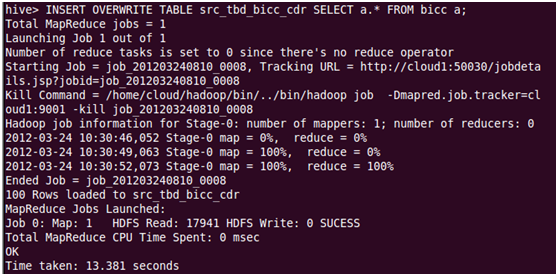
\includegraphics[]{photo/insert-bicc-hive.png}
\caption{src\_tbd\_bicc\_cdr表的插入时间}
\end{figure} 

\item 查看插入后的结果:
\clearpage
\begin{figure}[!ht]
\centering
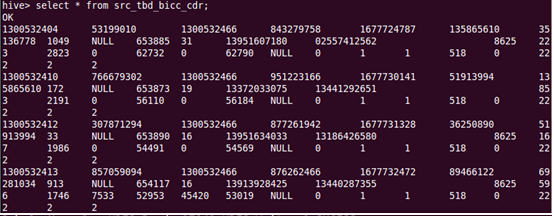
\includegraphics[]{photo/select-bicc-hive.png}
\caption{查看hive表}
\end{figure} 

再查看hbase表:
\begin{figure}[!ht]
\centering
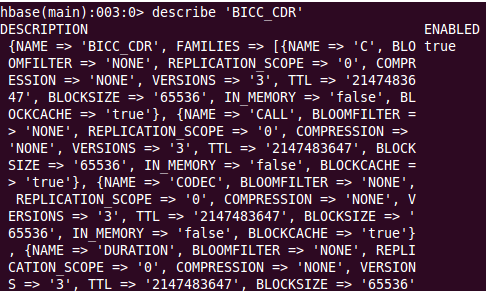
\includegraphics[]{photo/scan-bicc-hbase.png}
\caption{查看hbase表}
\end{figure} 

\end{enumerate}

同理可以对应于上述的大表yuyin和duanxin建立相应的表hbase\_yuyin和hbase\_duanxin。以下是它们插入数据所用的时间:
\clearpage

\begin{figure}[!ht]
\centering
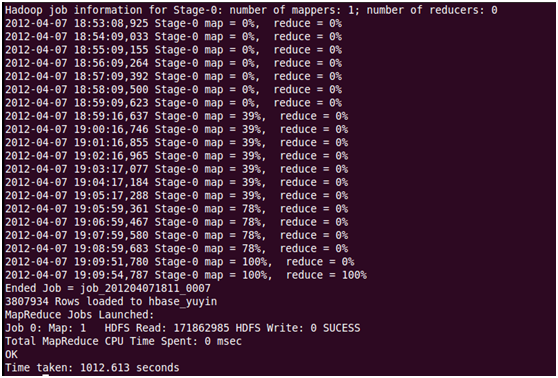
\includegraphics[scale=0.8]{photo/insert-yuyin-hbase.png} 
\caption{yuyin表的插入时间}
\end{figure} 

\begin{figure}[!ht]
\centering
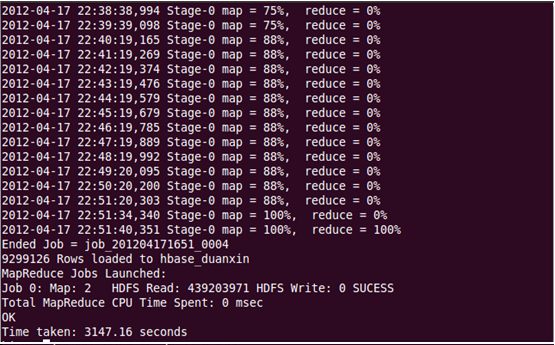
\includegraphics[scale=0.8]{photo/insert-duanxin-hbase.png}
\caption{duanxin表的插入时间}
\end{figure} 

\subsection{导入数据到mongoDB}
对于mongoDB来说,有其自带的导入工具mongoimport,这个工具的使用方法可以在官方的文档上找到\footnote{http://www.mongodb.org/display/DOCS/Import+Export+Tools\#ImportExportTools-mongoimport}。由于mongoDB面向文档,所以不用事先建立一个表,而是直接可以从文本文件中导入,需要制定相应的域就可以了。
这里给出我使用的例子:
\begin{lstlisting}
./mongoimport -d "mydb" -c "bicc" -f "start_time_s,start_time_ns,end_time_t,end_time_ns,cdr_index,source_ip,destination_ip,cic,opc,dpc,release_reason,calling_number,called_number,original_called_number,transfer_number,location_number,response_time,acm_time,anm_time,rel_time,call_duration,codec_modify_flag,codec_modify_result,codec_negotiation_flag,codec_negotiation_result,codec_type,call_type,is_ext_platform,call_hold,call_forward,call_waiting,conference_call" --type csv --file /mnt/hgfs/home/data/bicc_100.csv
\end{lstlisting}
数据量小时导入很快,当导入数据量很大时就需要消耗一定的时间。如下图所示:
\begin{figure}[!ht]
\centering
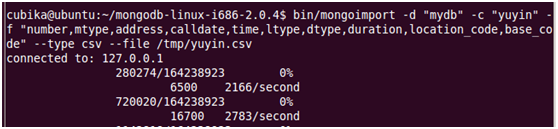
\includegraphics[]{photo/mongoimport.png} 
\caption{yuyin表的插入时间}
\end{figure} 
从图中可以看出整个导入过程花了3000秒左右。

\subsection{导入数据到mysql中}
导入时首先建立表,再进行插入。建表语句为:
\begin{lstlisting}[language=SQL]
create table duanxin
(
key int,
number string,
mtype int,
address string,
calldate string,
time string,
ltype int,
dtype int,
duration int,
location_code string,
base_code string
)
row format delimited 
fields terminated by '|'
stored as textfile;
\end{lstlisting}

插入语句为:
\begin{lstlisting}
LOAD DATA LOCAL INPATH '/home/cloud/data/ 清单数据/ 数据部分/duanxin2.txt' OVERWRITE INTO TABLE duanxin;
\end{lstlisting}